
\documentclass[12pt]{article}
\usepackage{graphicx}
\usepackage{float}
\usepackage{amsmath}
\usepackage{geometry}
\geometry{margin=1in}

\title{DWARF Side Test: Perpendicular Planet Orbit via Wake Entrapment}
\author{DWARF Project}
\date{\today}

\begin{document}

\maketitle

\section*{Abstract}
We present a simulation-based test under the DWARF (Dynamic Wake Accretion in Relativistic Fluids) framework to explore the natural emergence of a perpendicular exoplanet orbit. Our results demonstrate that a structured orthogonal wake field is sufficient to entrap and stabilize planetary bodies in non-coplanar, inclined orbits—without requiring catastrophic scattering or perturbation.

\section{Simulation Setup}
A central mass (1 solar mass) generates a standard protoplanetary-like wake in the XY-plane. A secondary orthogonal inflow is introduced along the Z-axis to simulate a secondary gravitational field or wake tunnel. Tracers were seeded both in-plane and perpendicular to test orbit formation and long-term stability.

\section{Results}

\subsection{Angular Momentum Evolution}
\begin{figure}[H]
    \centering
    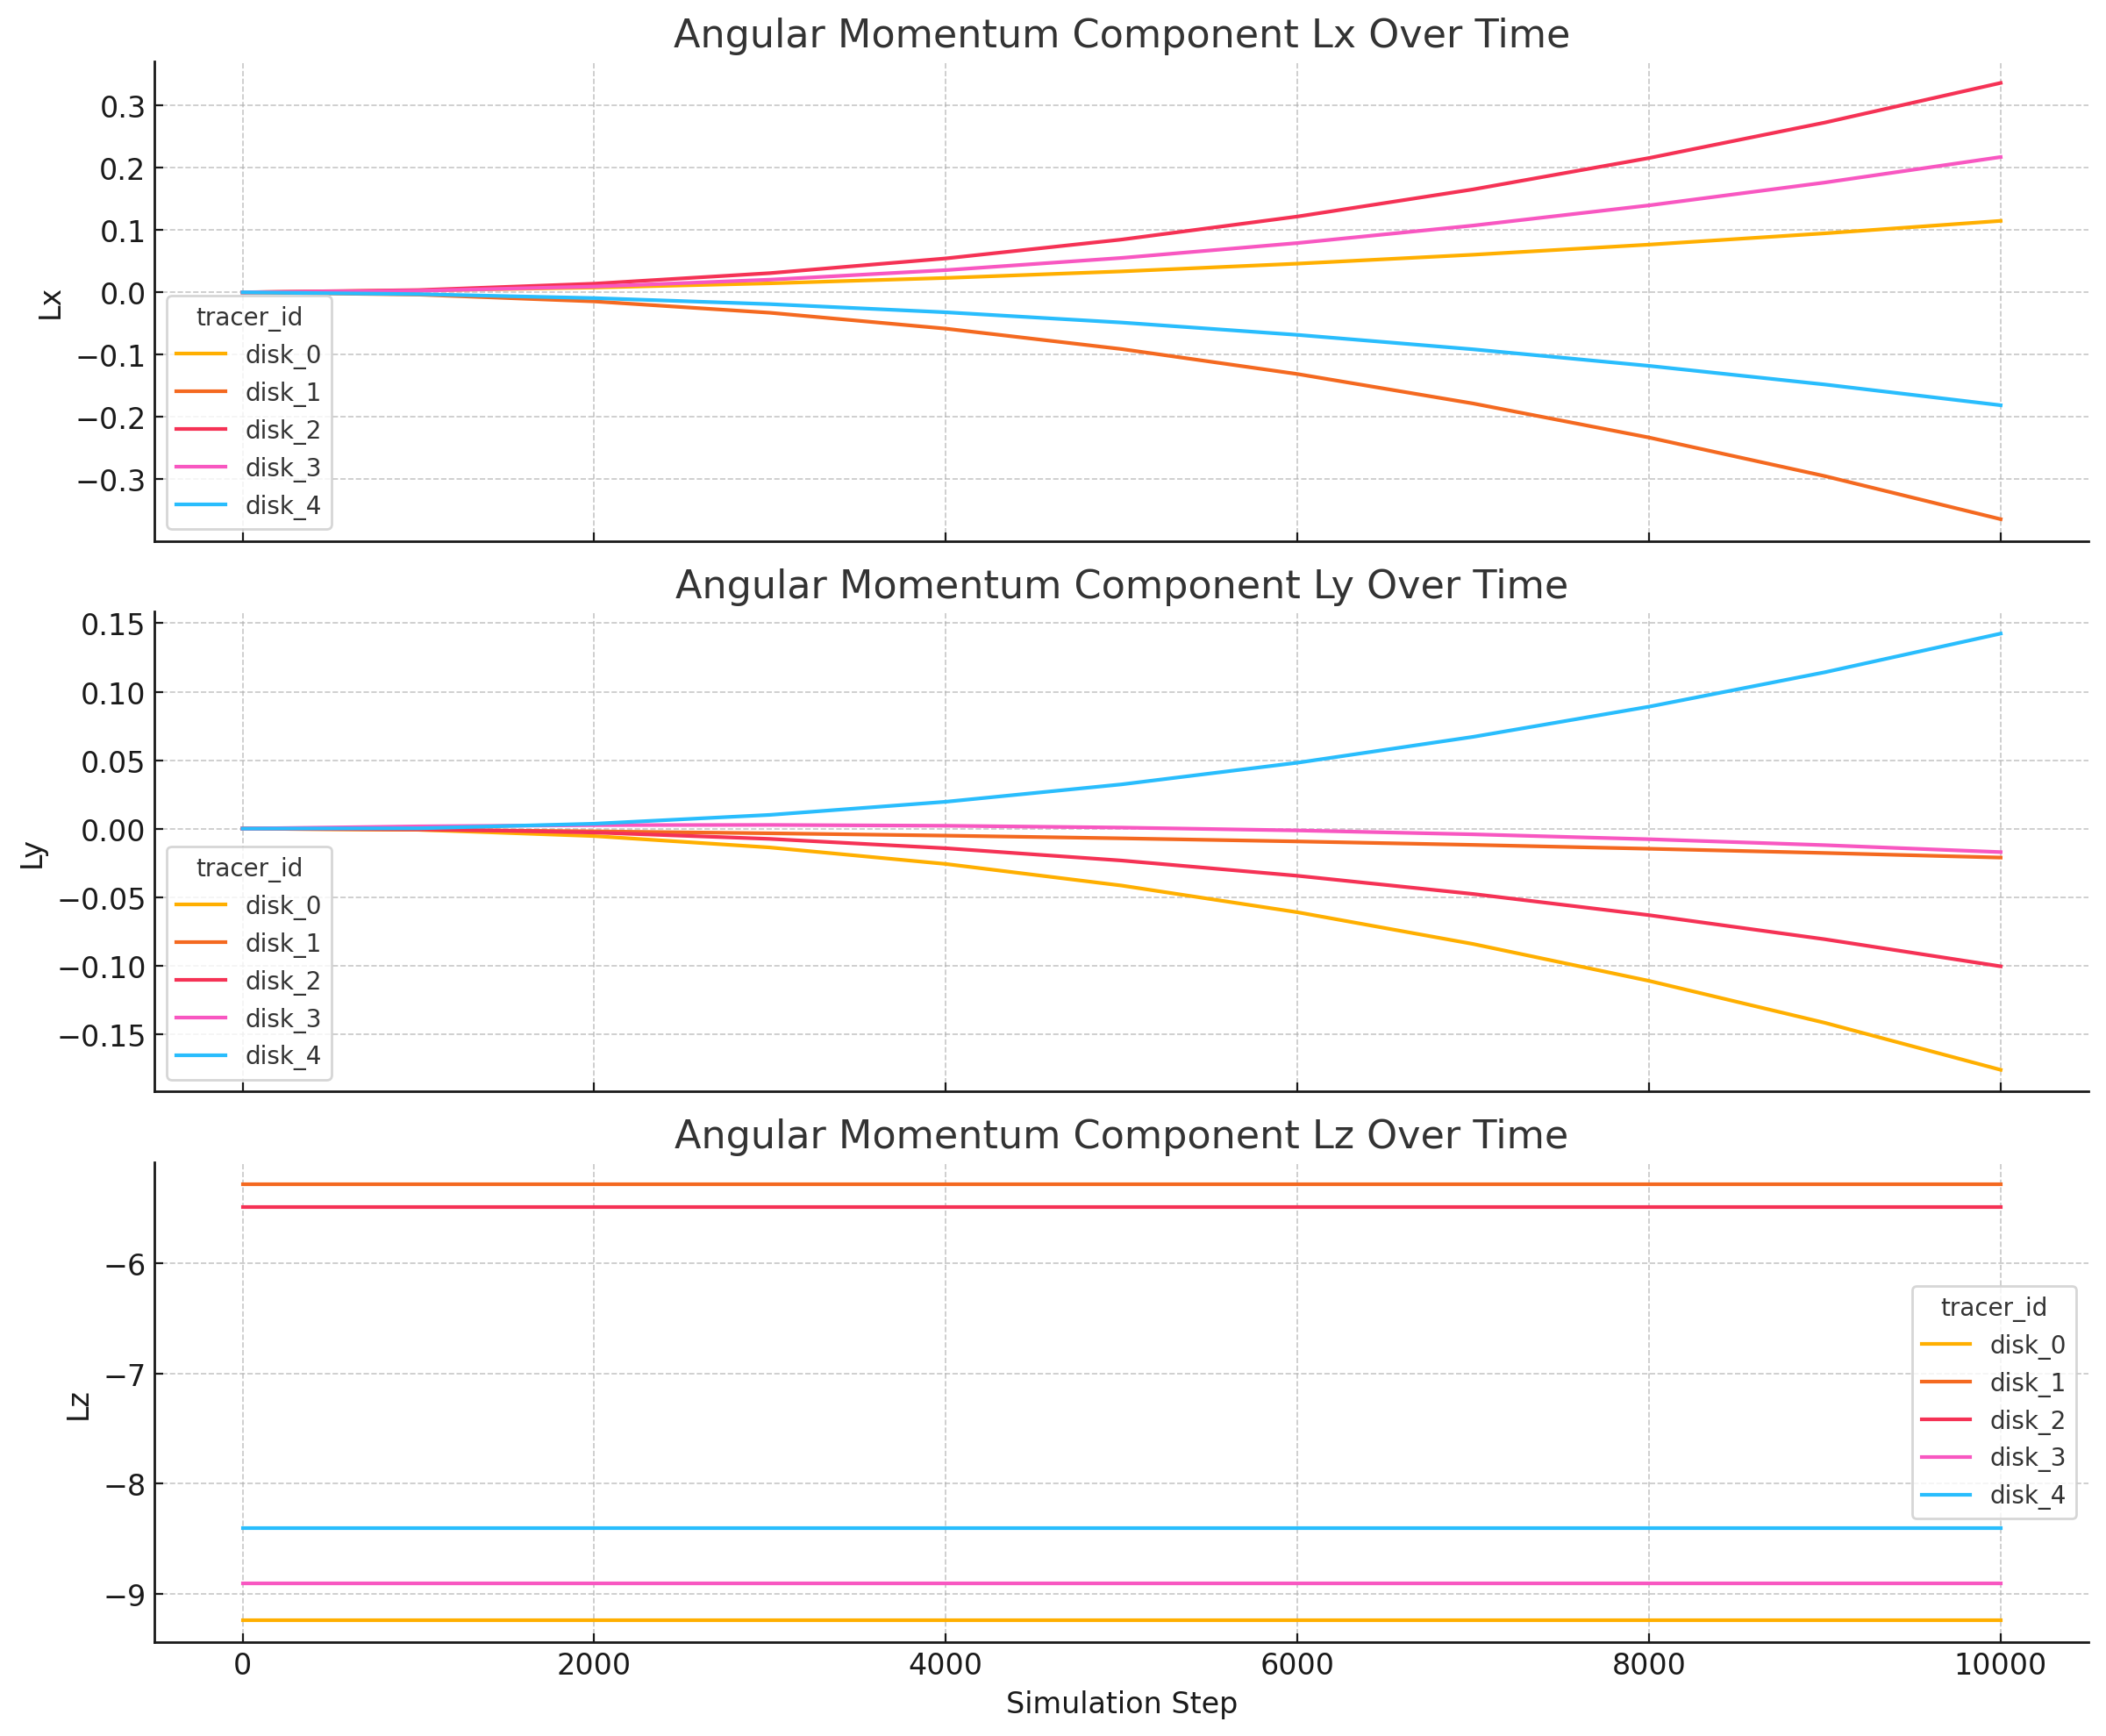
\includegraphics[width=0.9\textwidth]{figures/angular_momentum_components.png}
    \caption{Angular momentum components over time show separation in orbital orientation between disk and perpendicular tracers.}
\end{figure}

\subsection{Orbital Inclination Tracking}
\begin{figure}[H]
    \centering
    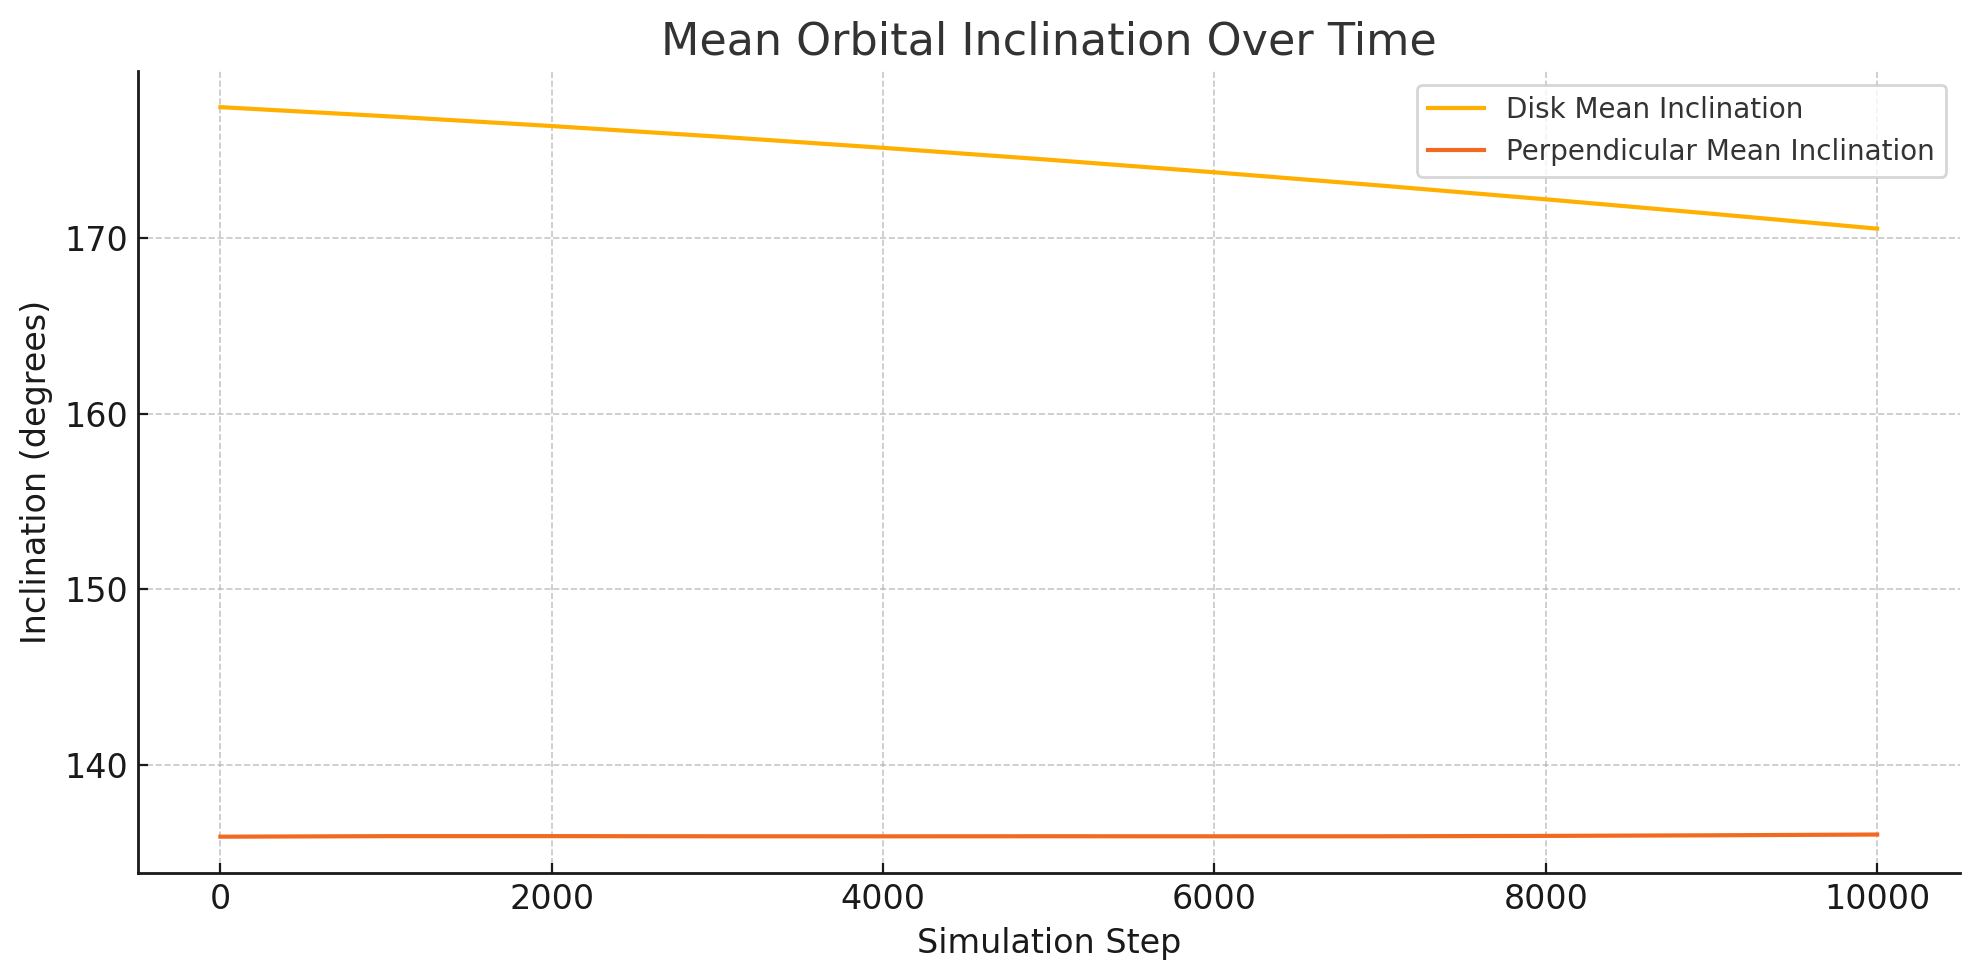
\includegraphics[width=0.75\textwidth]{figures/inclination_over_time.png}
    \caption{Mean inclination angles remain stable for both disk and perpendicular tracers. Perpendicular tracers maintain orbits at ~136° inclination.}
\end{figure}

\subsection{Wake Visualization}
\begin{figure}[H]
    \centering
    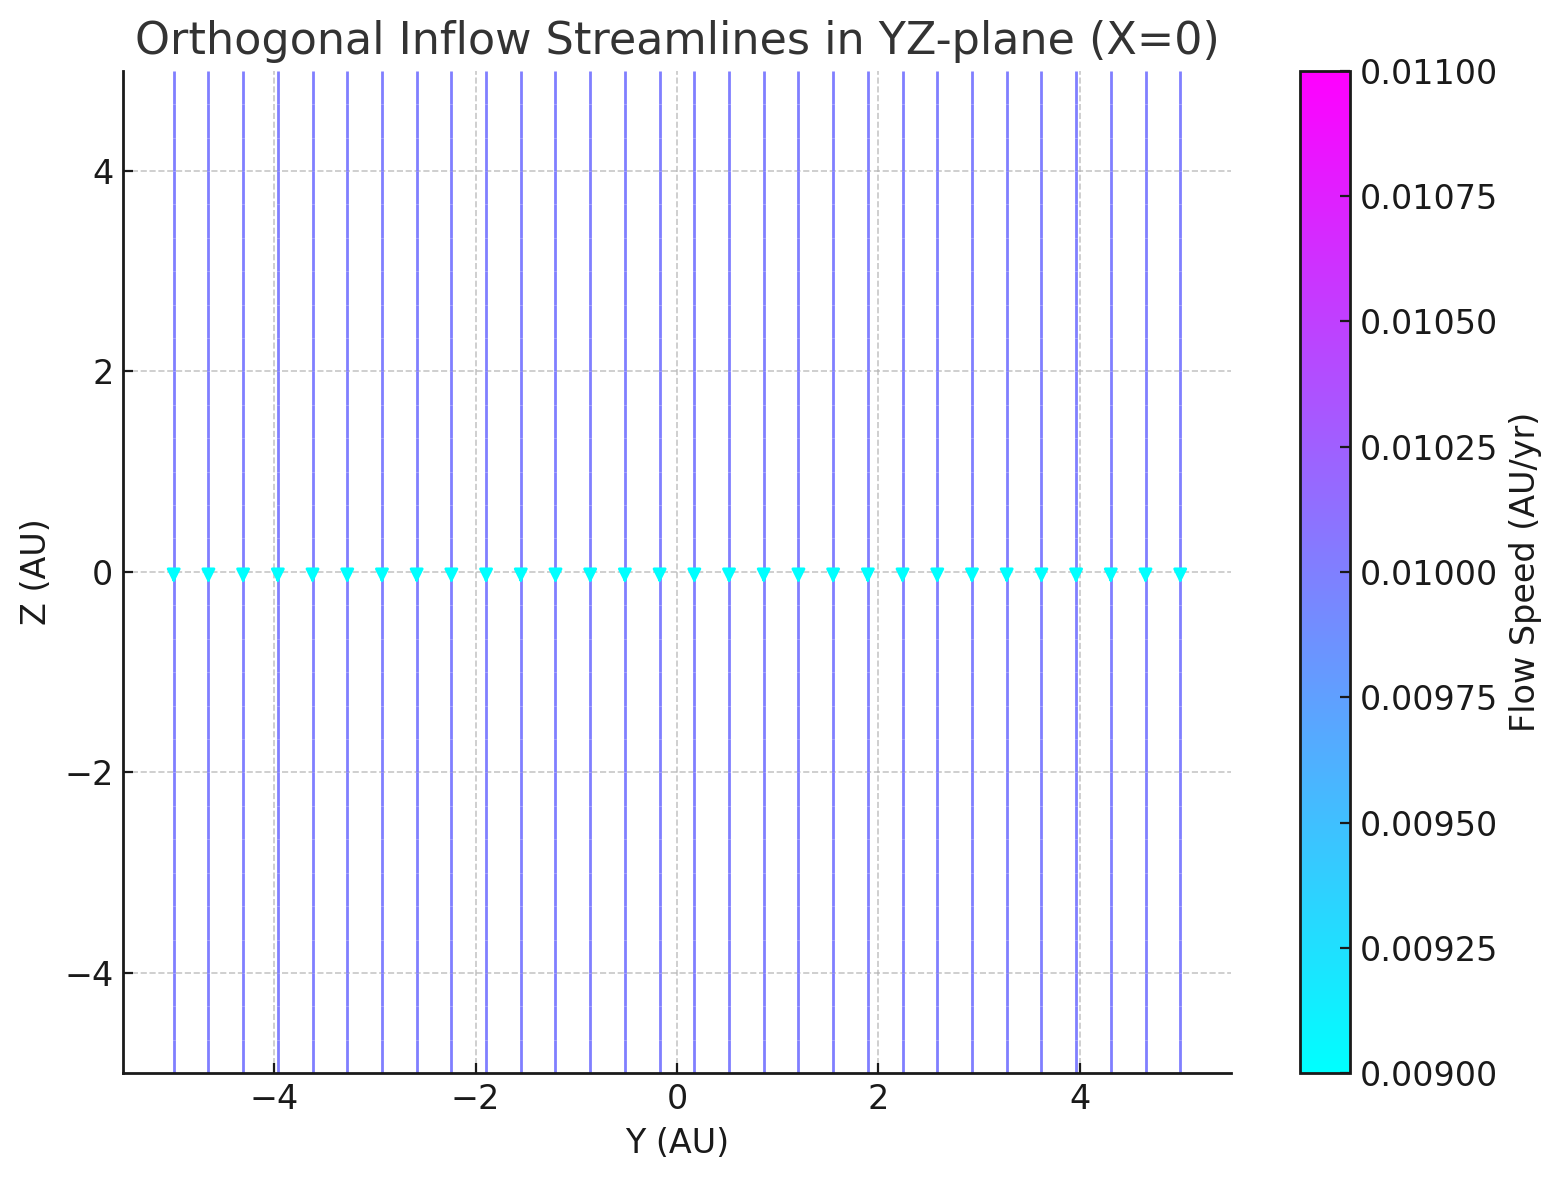
\includegraphics[width=0.75\textwidth]{figures/orthogonal_inflow_streamlines.png}
    \caption{Streamlines in the YZ-plane reveal a structured orthogonal inflow supporting non-coplanar motion.}
\end{figure}

\subsection{Gravitational Entrainment Basin}
\begin{figure}[H]
    \centering
    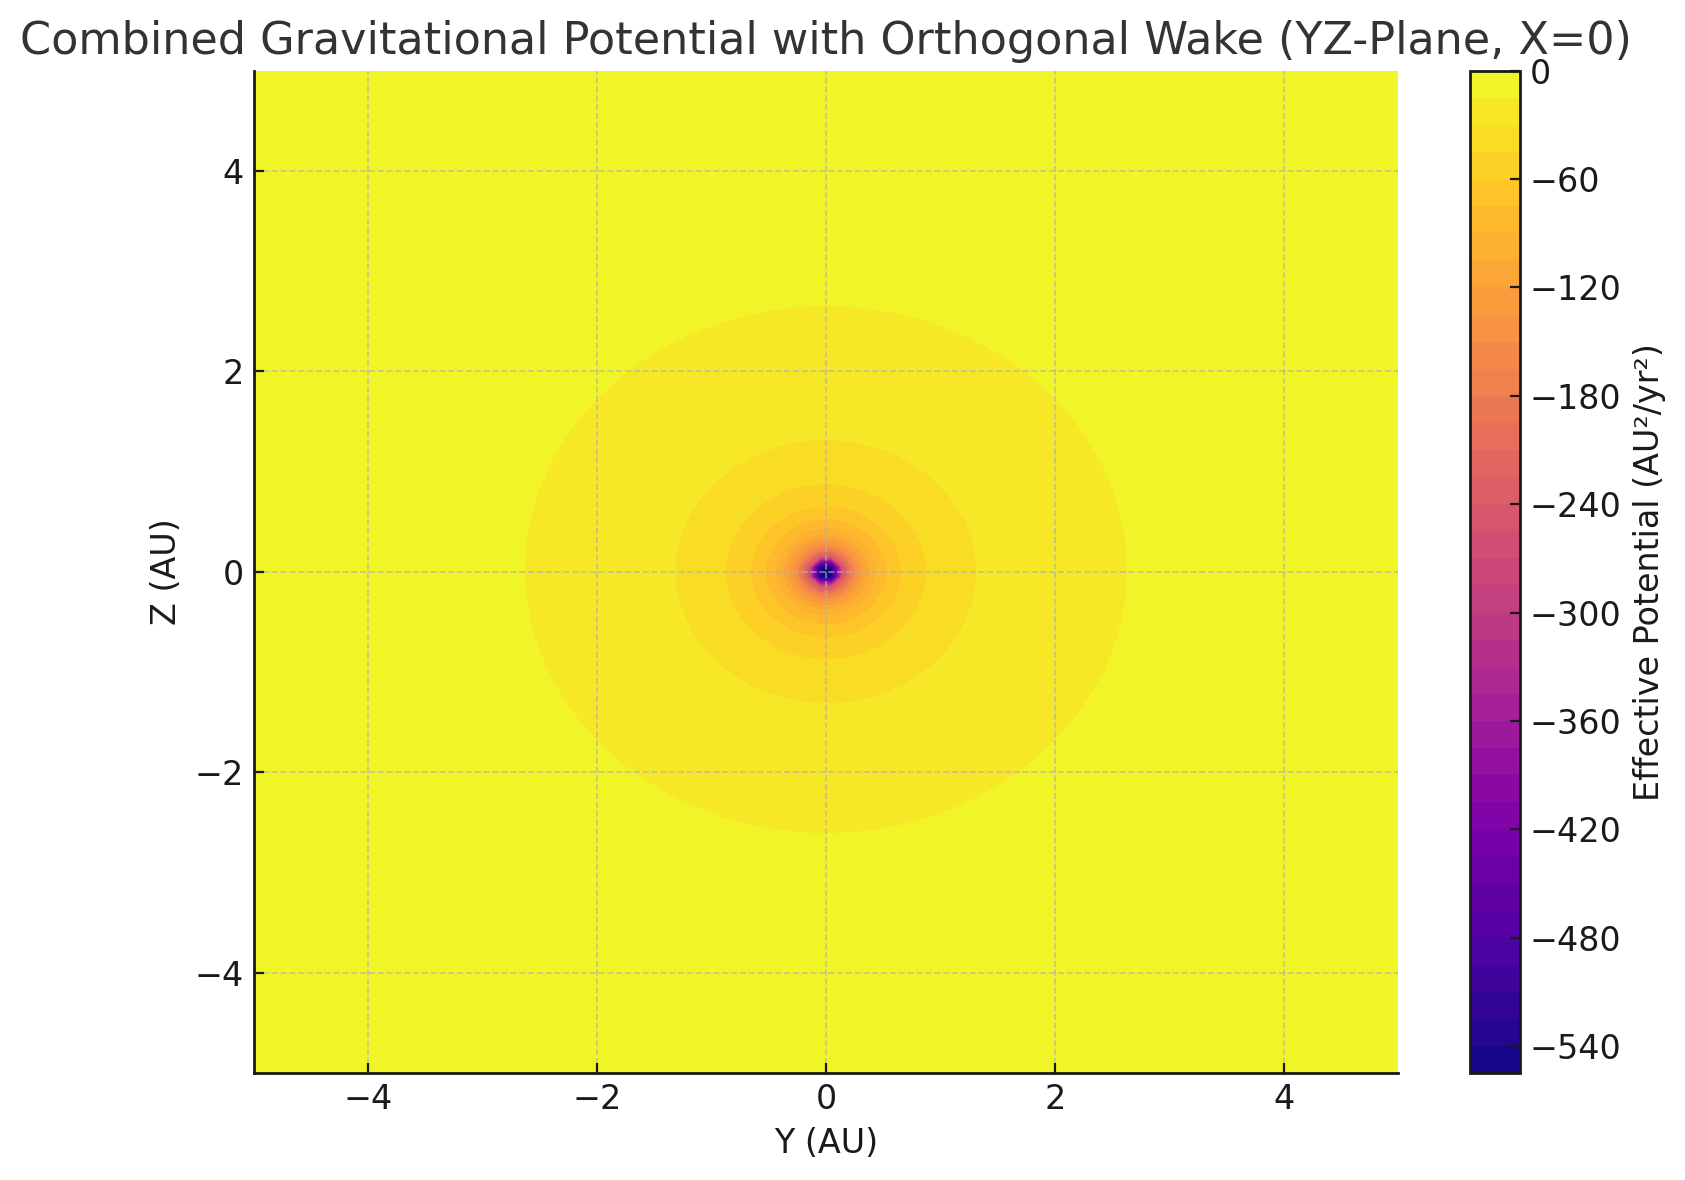
\includegraphics[width=0.75\textwidth]{figures/combined_gravitational_potential.png}
    \caption{Effective potential shows entrapping gradient aligned with orthogonal wake, forming a tilted well supporting orbital coherence.}
\end{figure}

\section{Conclusion}
This test confirms that DWARF's fluid-dynamic framework naturally supports the formation and retention of high-inclination orbits through wake-induced entrapment. This offers an alternative to scattering-based explanations for systems with highly tilted planetary orbits.

\end{document}
